\chapter{Empezando en la UDC}

\section{La tarjeta universitaria}

La \href{https://www.udc.es/es/tui/}{\textbf{\acrfull{TUI}}} acredita estudiantes, profesorado y personal de administración y servicios como miembros de la comunidad universitaria.

Además, con la \acrshort{TUI} es posible solicitar préstamos de libros de las bibliotecas de la \acrshort{UDC}, utilizar algunos servicios tecnológicos y beneficiarse de gran variedad de \href{https://www.udc.es/es/tui/guias_comerciais/}{\textbf{descuentos}}.

\begin{exampleBox}
    Con la \acrfull{TUI} es posible acceder gratuitamente a museos científicos coruñeses como el museo Domus, la Casa de las Ciencias o el Aquarium Finisterrae.
\end{exampleBox}

El \textbf{proceso de obtención} de la \acrshort{TUI} está detallado en la página web de la \href{https://www.udc.es/es/tui/emision/}{\acrshort{UDC}}

\begin{curiosityBox}
    Con el objetivo de reducir la huella ecológica provocada por el uso excesivo del plástico, la \acrshort{UDC} convirtió la tarjeta universitaria a un formato digital disponible a través de \texttt{UDC.gal}, la aplicación oficial de la \acrshort{UDC}.\\

    Únicamente puede seguir obteniendo la tarjeta de plástico el personal que necesite la tarjeta criptográfica para la firma electrónica, controles de acceso basados en tarjeta de proximidad o que no disponga de un teléfono compatible.
\end{curiosityBox}


\section{El correo electrónico}

El correo electrónico institucional universitario es una dirección de correo proporcionada por la universidad a sus estudiantes, profesores, y personal administrativo.

Es la \textbf{principal vía de comunicación entre la universidad y sus miembros}. A través de él, se envían avisos importantes, como convocatorias, actualizaciones académicas, fechas de exámenes, eventos, y otras informaciones oficiales.

Además la dirección de correo actúa como una \textbf{credencial de identificación} que permite acceder a otros recursos y servicios de la universidad.

\begin{curiosityBox}
    En las direcciones de correo electrónico de la \acrshort{UDC} pueden utilizarse tanto los dominios \textbf{\texttt{@udc.es}} como \textbf{\texttt{@udc.gal}}. Para algunas cosas, como puede ser crear cuentas en páginas con las que la \acrshort{UDC} tenga convenios, puede que solo funcione el dominio \texttt{@udc.es}.
\end{curiosityBox}

\begin{rememberBox}
    El correo electrónico permite utilizar \textbf{reglas} para \textbf{filtrar} y \textbf{catalogar} los mensajes. 
\end{rememberBox}

\subsection{Herramientas de Microsoft Office 365}

Con el \textbf{correo de la \acrshort{UDC}} es posible obtener gratuitamente las herramientas de \href{https://www.office.com/}{Office 365}.

\FloatBarrier
\begin{figure}[htp]
    \centering
    \frame{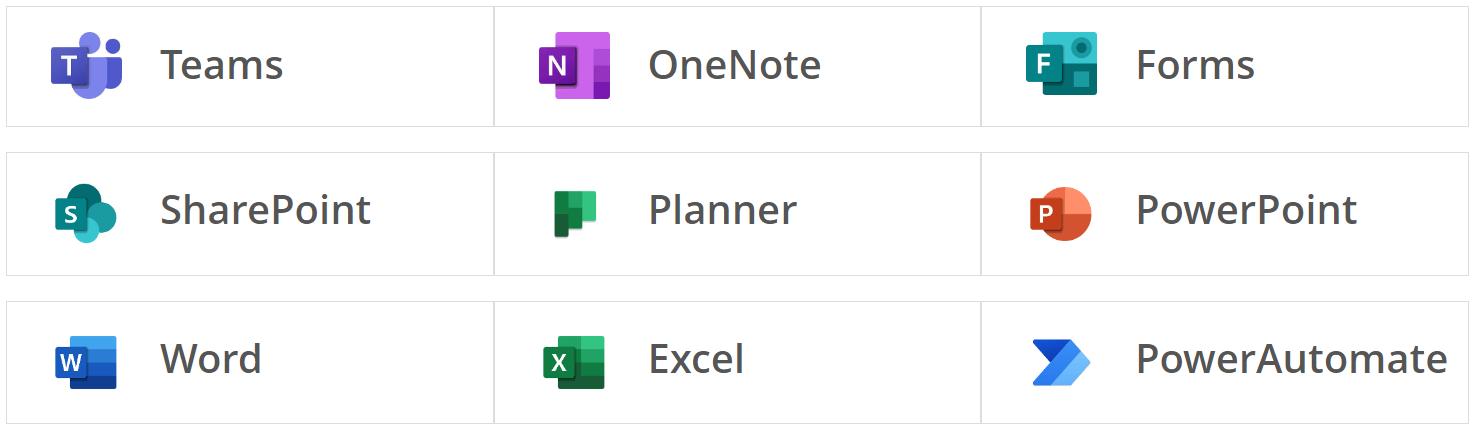
\includegraphics[width=0.6\linewidth]{figures/udc/Office365.png}}
\end{figure}
\FloatBarrier

Entre estas destaca \textbf{Microsoft Teams}, que es la principal plataforma de comunicación \textbf{entre los miembros} de la comunidad universitaria.


\section{Sitios web}

\subsection{Servizos UDC}

En \textbf{Servizos UDC} (\url{\linkServizosUDC}) es posible comprobar y modificar los datos personales, cambiar la fotografía del perfil, \textbf{cambiar la contraseña}, obtener un certificado de vinculación con la \acrshort{UDC} y acceder a otros sitios web de la \acrshort{UDC}.

\subsection{Espazos UDC}

En \textbf{Espazos UDC} (\url{\linkEspazosUDC}) se puede ver el \textbf{horario asignado} de las asignaturas, consultar las disponibilidades de los espacios del centro, ver los horarios de tutorías del profesorado y realizar reservas de espacios y equipo. 

\subsection{Secretaría Virtual}

En la \textbf{Secretaría Virtual} (\url{https://matricula.udc.es/Secretaria/}) se pueden comprobar los datos personales (los cuales pueden ser modificados en \href{\linkServizosUDC}{Servizos UDC}), consultar el \textbf{expediente}, realizar la \textbf{matrícula de continuación de estudios} y comprobar el estado de \textbf{liquidaciones} y \textbf{trámites}.

\subsection{Campus Virtual}

El \textbf{Campus Virtual} (\url{\linkCampusVirtual}) es una plataforma en la que aparecen las distintas \textbf{asignaturas} en las que el alumnado está matriculado y a las que el profesorado sube las diapositivas, los \textbf{apuntes} y los \textbf{enunciados} de las \textbf{prácticas} y \textbf{entregas}.

\subsection{Portal de estudios}

El \textbf{portal de estudios} (\url{\linkPortalEstudos}) permite acceder a información sobre los distintos estudios de \textbf{grados}, \textbf{másteres} y \textbf{doctorados}. Para cada estudio pueden comprobarse información como las salidas profesionales y académicas, el plan de estudios, el profesorado y resultados del estudio.
